%   The formal definition from the Gupta paper
%   Semantics of updates, Update safety
%   Supported changes

% \section*{Formal safety guarantees}
% \ShowTOC[]

\begin{frame}{Update correctness}%{A Sub-title is optional}
\begin{center}
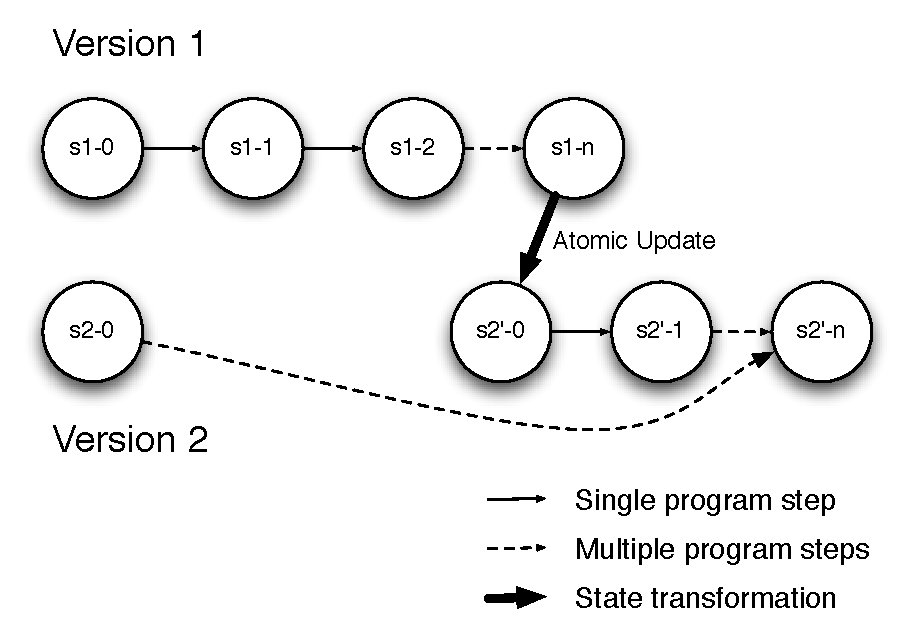
\includegraphics[scale=0.71]{images/gupta-state-graph}
\end{center}
\end{frame}

\begin{frame}{Correct update semantics}%{A Sub-title is optional}
Update correctness depends on semantics of application and state
transformers
\begin{itemize}
\item Transformer that initializes all variables to ``unknown'' is
      equivalent to restarting the program. Not useful.
\item When going from an 8-bit to 16-bit counter, no correct transformer
      exists
\end{itemize}
\end{frame}

\begin{frame}{Safety Guarantees}%{A Sub-title is optional}
\begin{itemize}
\item Correctness
  \begin{itemize}
  \item Showing an update correct is undecidable
  \item Rely on programmer and testing process for semantics and safety of
        update
  \end{itemize}
\item Well-formed updates
  \begin{itemize}
  \item All data accesses and method calls in the program respect language
        semantics.
  \item Type safety
  \end{itemize}
\end{itemize}
\end{frame}
